\section{Versuchsaufbau/-durchführung}
Zur experimentellen Überprüfung der Bragg-Bedingung sowie der quantitativen Untersuchung der Spektren wird der Aufbau nach Abbildung
\ref{fig: aufbau} verwendet. Die Apparatur besteht im Wesentlichen aus einer Kupferröntgenröhre, einem schwenkbaren \ce{LiF}-Kristall
und einem ebenfalls schwenkbaren Geiger-Müller-Zählrohr, das zum Nachweis der einfallenden Strahlungsintensität verwendet wird.
Weiter ist es möglich verschiedene Absorbermaterialien vor das Geiger-Müller-Zählrohr
zu montieren. Die zeitliche Justage der Drehwinkel, sowei die Datenaufnahme erfolgt computergesteuert mit einer
Messsoftware. Der Aufbau ermöglicht somit eine Untersuchung der Intensität in Abhängigkeit von der Energie
der Röntgenstrahlung.
\begin{figure}
  \centering
  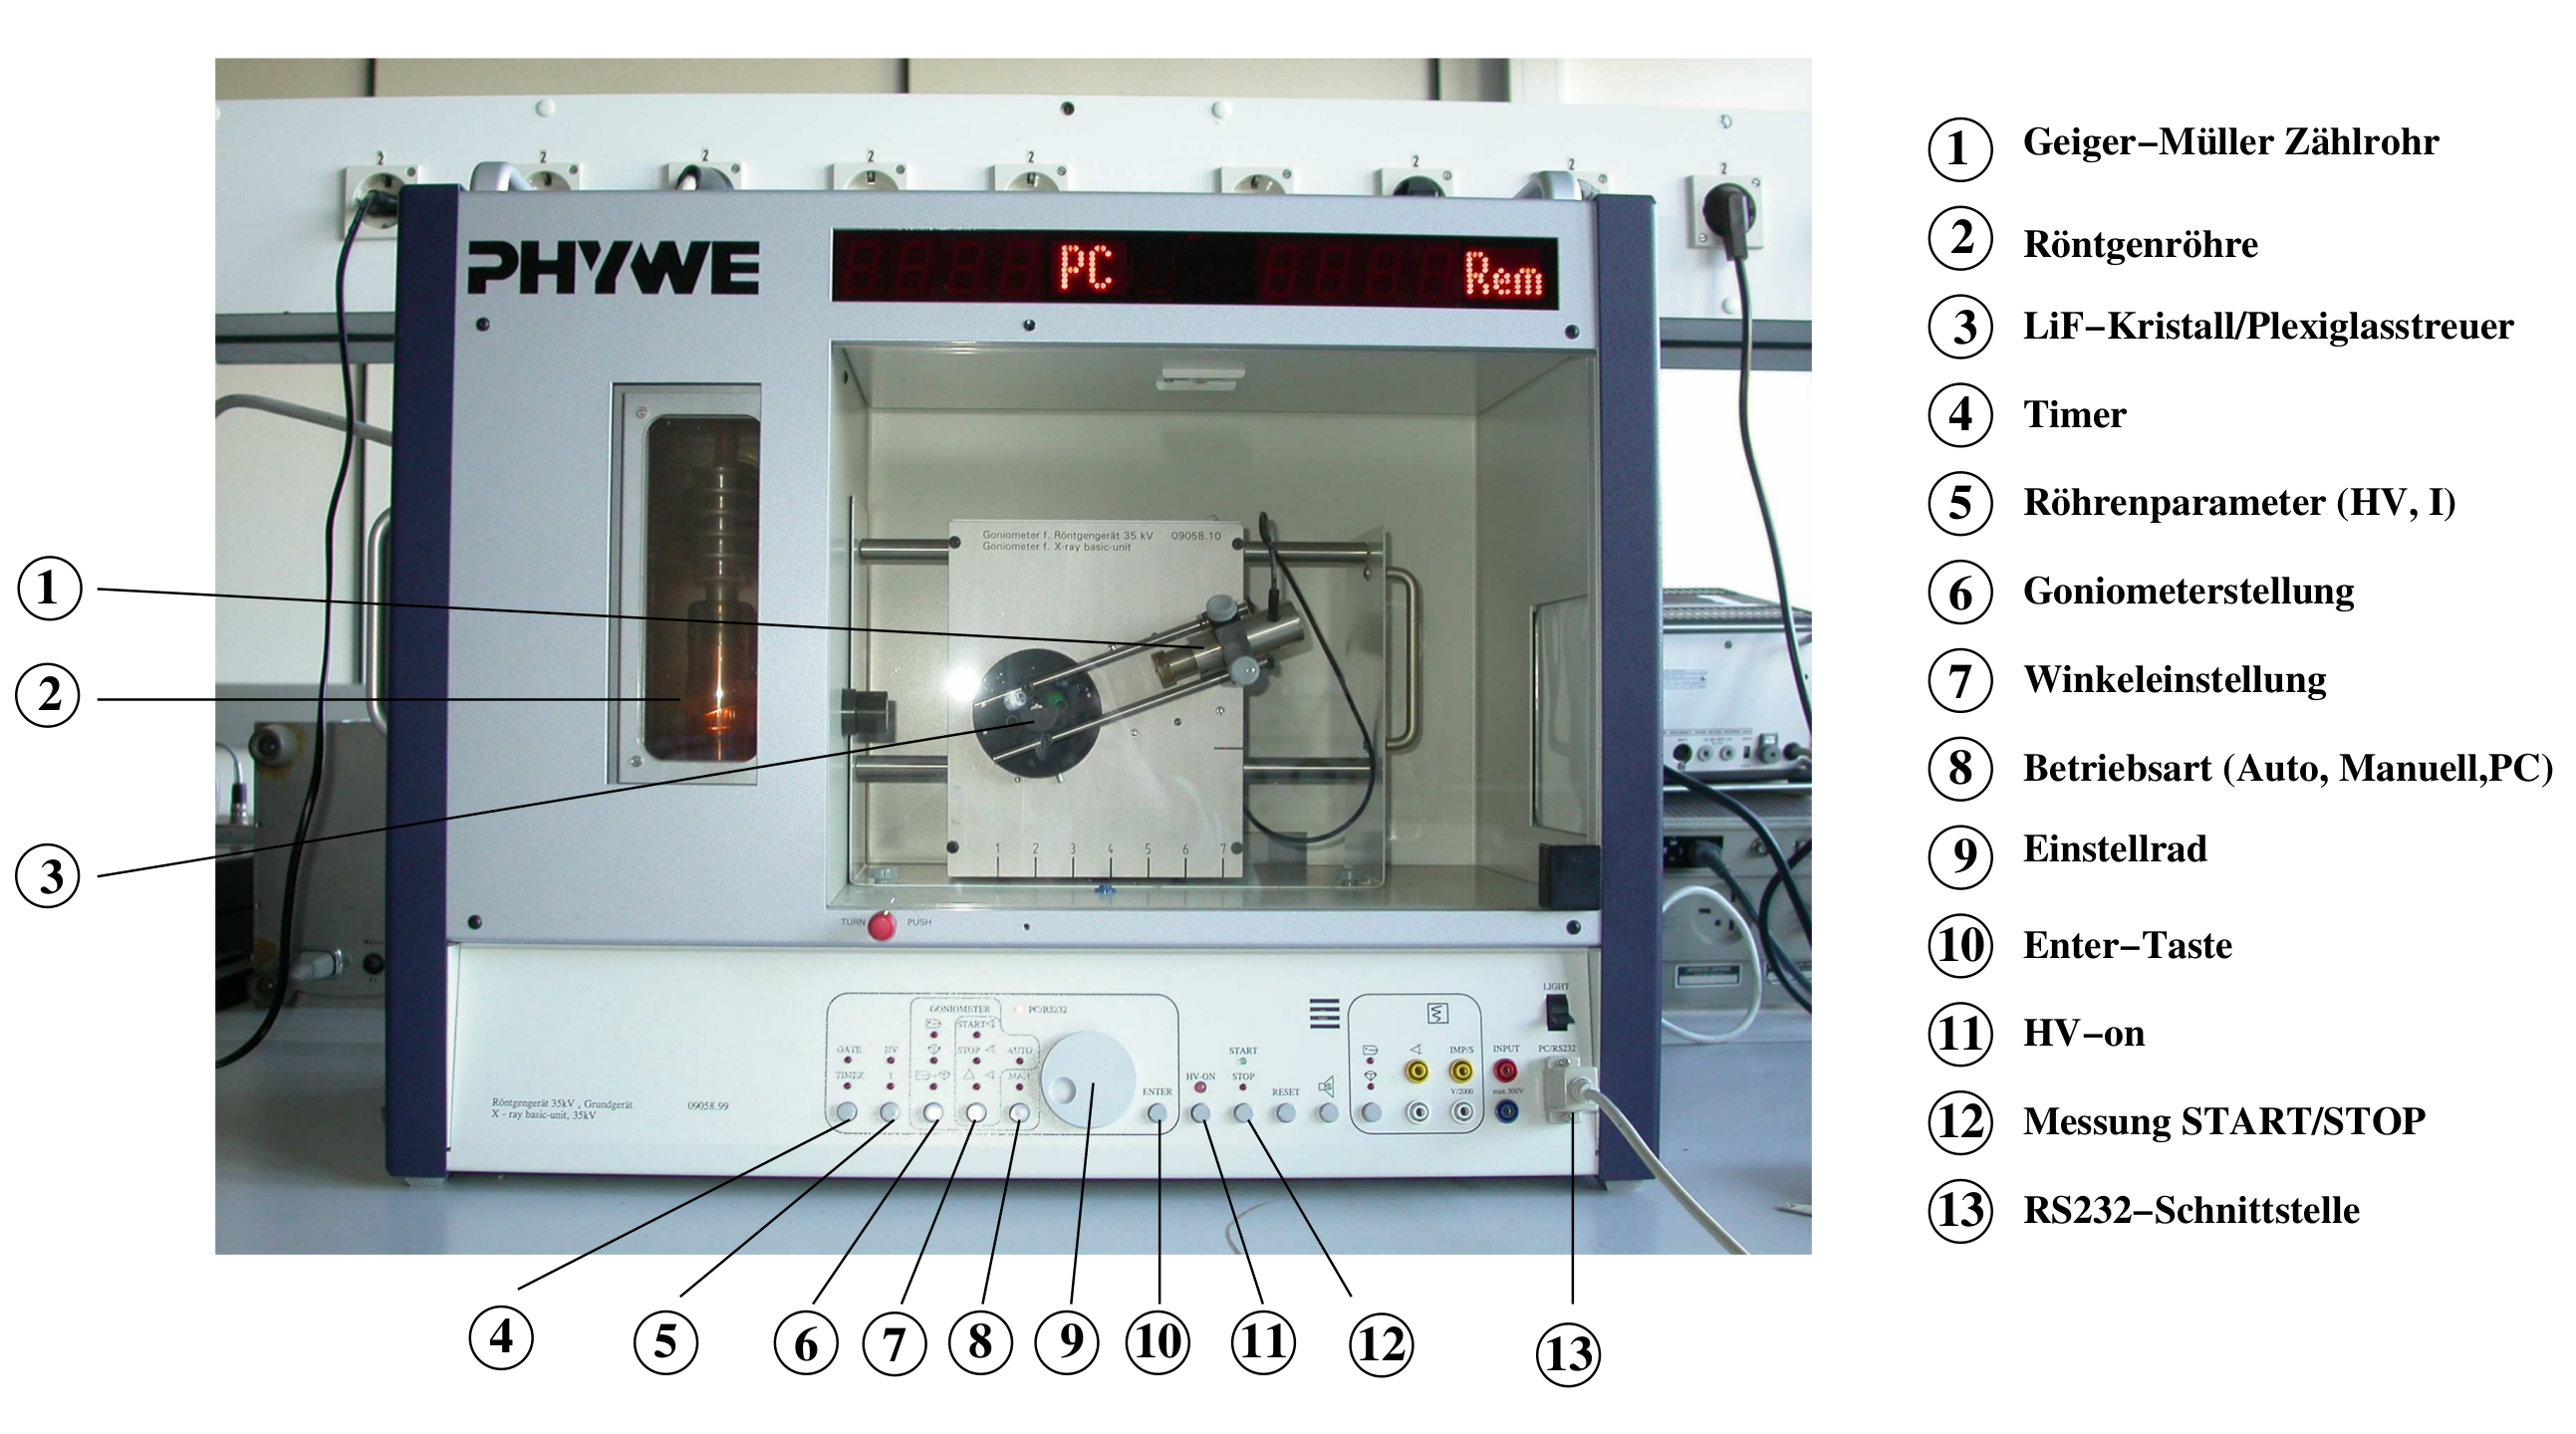
\includegraphics[width = 0.8\textwidth]{pics/aufbau.png}
  \caption{Darstellung der verwendeten Messaparatur zur Untersuchung von Röntgenemission und -absorption \cite{anleitung602}.}
  \label{fig: aufbau}
\end{figure}
\subsection{Überprüfung der Bragg-Bedingung}
Der Kristallwinkel wird auf den konstanten Wert $\SI{14}{\degree}$ eingestellt. Der Winkel des Zählrohrs wird im Winkelbereich
von $\SI{26}{\degree}$ - $\SI{30}{\degree}$ mit einem Winkelzuwachs von $\SI{0.1}{\degree}$ und einer Integrationszeit
von $\SI{5}{\second}$ variiert. Die Betrachtung der Lage des Maximums der so aufgenommenen Intensitätsverteilung ermöglicht eine Überprüfung
der Bragg-Bedingung \eqref{eq: bragg}.

\subsection{Emissionspektrum}
Das Emissionspektrum der verwendeten \ce{Cu}-Röntgenröhre wird für eine zeitliche Variation des Glanzwinkels
$\SI{4}{\degree} \leq \theta \leq \SI{26}{\degree}$ in Schritten von $\SI{0.2}{\degree}$ und einer Integrationszeit
von $\SI{5}{\second}$ aufgezeichnet. Die so bestimmten Daten ermöglichen die Untersuchung der $K\ua{\alpha}$- bzw.
$K\ua{\beta}$-Linie und eine qualitative Diskussion des kontinuierlichen Bremsspektrums.

\subsection{Absorptionsspektrum}
Das Röntgenabsorptionsspektrum wird für fünf Materialen mit Kernadungszahl im Bereich $Z \in \left[30, 50 \right]$ und eine
mit $Z \geq 70$ untersucht. Hierzu wird jeweils eine Probe in den Aufbau integriert und die Beugungsintensität in Abhängigkeit
vom Glanzwinkel aufgezeichnet (Schrittweite $\SI{0.1}{\degree}$, Integrationszeit $\SI{20}{\second}$).
Ein geeigneter Winkelbereich wird jeweils anhand der Literaturwerte für die Lage der $K$-Kante gewählt.
